%=============================================================================
%  Rapport hebdomadaire de stage -- Semaines 6 et 7
%  Projet : Simulateur de controleur aerien -- copilote IA pour le controle aerien
%  Auteur : Nicolas Marano -- URCA / supercalculateur ROMEO (NVIDIA GH200)
%  Compilation : pdflatex (x2 pour la table des matieres)
%=============================================================================
\documentclass[11pt,a4paper]{article}

\usepackage[utf8]{inputenc}
\usepackage[T1]{fontenc}
\usepackage[french]{babel}
\usepackage{lmodern}
\usepackage{microtype}
\usepackage[a4paper,margin=2.3cm,headheight=15pt]{geometry}
\usepackage{graphicx}
\usepackage{booktabs}
\usepackage{array}
\usepackage[table]{xcolor}
\usepackage{titlesec}
\usepackage{enumitem}
\usepackage{caption}
\usepackage{fancyhdr}
\usepackage{listings}
\usepackage[most]{tcolorbox}
\usepackage{hyperref}

%--- Couleurs ----------------------------------------------------------------
\definecolor{atcblue}{RGB}{11,61,145}
\definecolor{atcteal}{RGB}{13,110,124}
\definecolor{atcgreen}{RGB}{22,128,71}
\definecolor{atcred}{RGB}{197,32,38}
\definecolor{atcpurple}{RGB}{109,40,180}
\definecolor{atcslate}{RGB}{71,85,105}
\definecolor{lightgray}{RGB}{244,246,249}
\definecolor{rulegray}{RGB}{210,216,224}

\hypersetup{colorlinks=true, linkcolor=atcblue, urlcolor=atcteal, citecolor=atcblue,
  pdftitle={Rapport de stage -- Semaines 6 et 7}, pdfauthor={Nicolas Marano}}

%--- Titres ------------------------------------------------------------------
\titleformat{\section}{\Large\bfseries\color{atcblue}}{\thesection}{0.6em}{}
\titleformat{\subsection}{\large\bfseries\color{atcteal}}{\thesubsection}{0.6em}{}
\titleformat{\subsubsection}{\normalsize\bfseries\color{atcteal}}{\thesubsubsection}{0.5em}{}
\titlespacing*{\section}{0pt}{16pt}{8pt}

%--- En-tete / pied de page --------------------------------------------------
\pagestyle{fancy}
\fancyhf{}
\renewcommand{\headrulewidth}{0.4pt}
\renewcommand{\footrulewidth}{0.4pt}
\fancyhead[L]{\small\color{atcblue}\itshape Copilote IA pour le controle aerien}
\fancyhead[R]{\small\color{atcblue}\itshape Semaines 6 \& 7}
\fancyfoot[L]{\small Nicolas Marano, URCA / ROMEO}
\fancyfoot[R]{\small\thepage}

%--- Boites tcolorbox --------------------------------------------------------
\newtcolorbox{objbox}{enhanced, colback=lightgray, colframe=atcblue,
  boxrule=0.8pt, arc=3pt, left=10pt, right=10pt, top=8pt, bottom=8pt,
  fonttitle=\bfseries\color{white}, coltitle=white, colbacktitle=atcblue,
  title={Objectif de la semaine}}

\newtcolorbox{resbox}{enhanced, colback=atcgreen!6, colframe=atcgreen,
  boxrule=0.8pt, arc=3pt, left=10pt, right=10pt, top=8pt, bottom=8pt,
  fonttitle=\bfseries, coltitle=white, colbacktitle=atcgreen,
  title={Resultats cles}}

\newtcolorbox{warnbox}{enhanced, colback=atcslate!6, colframe=atcslate,
  boxrule=0.8pt, arc=3pt, left=10pt, right=10pt, top=8pt, bottom=8pt,
  fonttitle=\bfseries, coltitle=white, colbacktitle=atcslate,
  title={Contraintes techniques et choix d'ingenierie}}

%--- Style des listings ------------------------------------------------------
\lstdefinestyle{atccode}{
  basicstyle=\ttfamily\footnotesize,
  backgroundcolor=\color{lightgray},
  frame=single, framesep=5pt, rulecolor=\color{rulegray},
  breaklines=true, breakatwhitespace=true,
  showstringspaces=false,
  keywordstyle=\color{atcblue}\bfseries,
  commentstyle=\color{atcgreen}\itshape,
  stringstyle=\color{atcpurple},
  numberstyle=\tiny\color{gray},
  columns=fullflexible, keepspaces=true,
  aboveskip=8pt, belowskip=8pt,
}
\lstset{style=atccode}

\setlist[itemize]{label=\textbullet, leftmargin=1.4em, itemsep=2pt, topsep=3pt}
\captionsetup{font=small, labelfont={bf,color=atcblue}}
\renewcommand{\arraystretch}{1.25}

%=============================================================================
\begin{document}

%--- Page de garde -----------------------------------------------------------
\begin{titlepage}
\centering
\vspace*{1.2cm}
{\color{atcblue}\rule{\textwidth}{2pt}}\\[0.5cm]
{\Huge\bfseries\color{atcblue} Rapport d'avancement de stage\par}
\vspace{0.35cm}
{\LARGE\color{atcteal} Semaines 6 \& 7\par}
\vspace{0.25cm}
{\large Synthese vocale par clonage de voix (XTTS) \\[2pt]
et integration : la requete unifiee vers un JSON exploitable\par}
\vspace{0.4cm}
{\color{atcblue}\rule{\textwidth}{2pt}}\\[1.0cm]

{\large\itshape Un copilote d'intelligence artificielle pour le controle aerien\par}
\vspace{1.6cm}

\begin{tabular}{rl}
\large\bfseries Auteur & \large Nicolas Marano\\[4pt]
\large\bfseries Projet & \large Simulateur de controleur aerien (PoC, 10 semaines)\\[4pt]
\large\bfseries Etablissement & \large Universite de Reims Champagne-Ardenne (URCA)\\[4pt]
\large\bfseries Calcul (IA) & \large Supercalculateur ROMEO : NVIDIA GH200 (Grace-Hopper, aarch64)\\[4pt]
\large\bfseries Domaine & \large Intelligence artificielle \& controle du trafic aerien\\[4pt]
\large\bfseries Periode & \large Semaines 6 et 7 du stage\\
\end{tabular}

\vfill
\begin{tcolorbox}[colback=lightgray, colframe=atcblue, arc=3pt, width=0.92\textwidth, center,
  left=12pt, right=12pt, top=8pt, bottom=8pt]
\small\centering
\textbf{Resume.} Ces deux semaines couvrent l'achevement de la boucle de dialogue
puis le debut de son integration. La semaine~6 ajoute le module de synthese vocale :
un clonage de voix \emph{zero-shot} (XTTS-v2) genere a la volee une voix distincte par
pilote virtuel, suivie d'une degradation VHF (filtre de Butterworth 300--3400~Hz) qui
reproduit le canal radio ; la synthese est mesuree a 3,9~s par collationnement et le
taux d'erreur mots de re-transcription de la voix synthetisee est de 22 a 24~\%. La
semaine~7 construit une \emph{requete unifiee} qui assemble la transcription, les
regles du RAG et une situation spatiale fixe pour produire un JSON conforme decrivant
l'action ; une chaine de validation deterministe garantit que ce JSON reste propre et
exploitable.
\end{tcolorbox}
\vspace{0.6cm}
{\small Annee universitaire 2025--2026}
\end{titlepage}

%--- Table des matieres ------------------------------------------------------
\tableofcontents
\thispagestyle{fancy}
\vspace{1cm}

%=============================================================================
\section{Contexte et positionnement des deux semaines}
%=============================================================================

Le projet automatise le dialogue radio pilote~/~controleur a l'interieur d'un
simulateur de trafic aerien. Une instruction parlee est transcrite, ancree dans la
phraseologie OACI, transformee en une commande validee, executee dans le simulateur
BlueSky, puis restituee en voix de pilote synthetisee. La chaine cible se resume
ainsi :

\begin{center}
\fbox{\parbox{0.95\textwidth}{\centering\ttfamily\footnotesize
voix pilote (VHF) $\rightarrow$ Whisper STT $\rightarrow$ NER + LLM avec RAG (OACI Doc 4444)
$\rightarrow$ JSON valide\\
$\rightarrow$ simulateur BlueSky (manoeuvre avion) $\rightarrow$ voix de readback synthetisee $\rightarrow$ boucle}}
\end{center}

Les semaines precedentes ont produit le module de \textbf{perception} (semaine~4,
reconnaissance vocale par Whisper fine-tune) et le module d'\textbf{interpretation}
par RAG (semaine~5, LLM ancre produisant un JSON valide et borne par une validation de
securite). Les semaines~6 et~7 couvrent deux progressions complementaires. La
semaine~6 ajoute le \textbf{dernier maillon} de la chaine, la \textbf{restitution
vocale} : l'aeronef ne se contente plus d'executer la manoeuvre, il repond sur la
frequence dans une voix qui lui est propre. La semaine~7 ouvre la phase
d'\textbf{integration} : plutot que de traiter chaque entree isolement, le systeme
reunit la transcription, les regles de phraseologie et une representation de l'espace
aerien au sein d'une \textbf{requete unifiee}. Le projet passe ainsi de la
construction de modules isoles a leur assemblage.

\subsection{Synthese chiffree des deux semaines}

\begin{table}[h]
\centering
\small
\begin{tabular}{>{\raggedright}p{1.6cm} >{\raggedright}p{8.1cm} l}
\toprule
\rowcolor{lightgray}\textbf{Semaine} & \textbf{Indicateur} & \textbf{Resultat}\\
\midrule
S6 & Latence de synthese (par collationnement, CPU) & \textbf{3,9~s} (RTF 0,82)\\
S6 & WER de re-transcription de la voix synthetisee & \textbf{22 a 24~\%}\\
S6 & WER de reference sur voix humaine reelle (validation S4) & 6,7~\%\\
S6 & Voix de reference clonees (pilotes / controleur) & 3\\
S7 & Entrees combinees dans la requete unifiee & 3\\
S7 & Situation spatiale fixe (fixes / segments / separation) & 7 / 6 / 5~NM\\
S7 & JSON exploitable produit (40 transcriptions reelles) & \textbf{100~\%}\\
S7 & Couches de validation du JSON de sortie & 4\\
\bottomrule
\end{tabular}
\caption{Vue d'ensemble des resultats obtenus durant les semaines 6 et 7.}
\end{table}

%=============================================================================
\section{Semaine 6 : Synthese vocale par clonage de voix}
%=============================================================================

\begin{objbox}
Implementer une solution de \textbf{clonage vocal} permettant de generer a la volee
l'audio des differents pilotes virtuels. Chaque aeronef doit pouvoir prononcer son
collationnement avec une voix qui lui est propre, sans entrainement specifique par
locuteur, et dans un rendu sonore compatible avec le canal radio VHF du simulateur.
\end{objbox}

\subsection{Methode : clonage \emph{zero-shot} avec XTTS-v2}

La generation repose sur le modele \texttt{XTTS-v2} (paquet \texttt{coqui-tts}). Le
choix d'un clonage \emph{zero-shot} evite tout entrainement par locuteur : le modele
reproduit le timbre d'une voix a partir d'un seul extrait de reference de quelques
secondes, fourni au moment de la synthese. Cette approche permet d'attribuer une voix
distincte a chaque aeronef sans constituer de corpus dedie ni lancer de campagne
d'entrainement supplementaire, ce qui est adapte a la contrainte de calcul et de
stockage du cluster.

\begin{table}[h]
\centering
\small
\begin{tabular}{>{\raggedright}p{4.3cm} >{\raggedright}p{4.3cm} p{5.0cm}}
\toprule
\rowcolor{lightgray}\textbf{Composant} & \textbf{Valeur} & \textbf{Remarque}\\
\midrule
Modele & \texttt{XTTS-v2} (\texttt{coqui-tts}) & multilingue, clonage zero-shot\\
Strategie & clonage sans entrainement & voix clonee depuis un extrait de reference\\
Voix de reference & 3 extraits ATCO2 (4 a 9~s) & une voix par pilote virtuel\\
Frequence native & 24~kHz $\rightarrow$ 16~kHz & rééchantillonnage vers l'entree ASR\\
Langue & \texttt{en} & phraseologie anglaise\\
Materiel d'inference & CPU (noeud GH200) & contournement du bug cuFFT (GPU)\\
Post-traitement & degradation VHF 300--3400~Hz & rendu radio (\emph{sim-to-real})\\
\bottomrule
\end{tabular}
\caption{Configuration de la synthese vocale (semaine 6).}
\end{table}

\subsection{Chaine de synthese}

La fonction \texttt{synth()} enchaine quatre etapes deterministes apres la generation
XTTS : rééchantillonnage de 24~kHz vers 16~kHz (frequence d'entree du pipeline ASR),
normalisation d'amplitude pour eviter l'ecretage, puis degradation VHF. La sortie est
un signal mono 16~kHz directement consommable par le reste de la chaine.

\begin{center}
\fbox{\parbox{0.95\textwidth}{\centering\ttfamily\footnotesize
texte de readback (OACI) $\rightarrow$ XTTS-v2 (clonage, voix de reference)
$\rightarrow$ rééchantillonnage 24$\rightarrow$16 kHz\\
$\rightarrow$ normalisation $\rightarrow$ degradation VHF (Butterworth 300-3400 Hz)
$\rightarrow$ wav 16 kHz}}
\end{center}

\begin{lstlisting}[language=Python, caption={Coeur de la synthese : clonage XTTS puis post-traitement (extrait de \texttt{tts\_atc.py}).}]
wav = np.asarray(tts.tts(text=text, speaker_wav=ref_wav, language=language), dtype=np.float32)
wav16 = resample_poly(wav, FS, XTTS_SR).astype(np.float32)   # 24k -> 16k
peak = np.max(np.abs(wav16)) + 1e-9
if peak > 1.0:
    wav16 = wav16 / peak
if vhf:
    wav16 = preprocess_waveform(wav16, training=False)        # bande passante VHF 300-3400 Hz
\end{lstlisting}

\subsection{Generation du collationnement (phraseologie OACI)}

Le texte prononce n'est pas l'instruction brute mais un \emph{collationnement}
conforme a la phraseologie. Le module \texttt{readback.py} convertit les ordres JSON
en telephonie standard : chiffres epeles un a un (\texttt{niner} pour 9), indicatifs
en code telephonique (\texttt{AFR}~$\rightarrow$~\emph{air france}), points de
cheminement en alphabet OACI. Le sens d'un changement d'altitude (montee ou descente)
est determine en comparant la valeur cible a l'altitude courante de l'aeronef.

\begin{lstlisting}[caption={Exemple de collationnement genere a partir d'un ordre JSON.}]
Ordre : {callsign: AFR1234, action: ALT, value: 10000}  (avion au FL130)
Texte : "descend flight level one zero zero, air france one two three four"
\end{lstlisting}

\subsection{Voix de reference}

Les voix de reference sont extraites du corpus ATCO2 (jeu de test) par le module
\texttt{make\_pilot\_voices.py} : il selectionne trois segments courts (4 a 9~s, non
silencieux) qui servent de timbres a cloner. Chaque aeronef de la flotte se voit
attribuer une de ces voix, de sorte que des pilotes differents sonnent differemment
sur la frequence. L'usage d'extraits radio reels comme reference contribue au realisme
du rendu.

\subsection{Degradation VHF et coherence de domaine}

La voix synthetisee par XTTS est propre (large bande). Pour la rendre credible sur une
frequence aeronautique, la chaine applique la degradation VHF deja validee en
semaine~2 : un filtre passe-bande de Butterworth d'ordre~6, limite a la bande
300--3400~Hz (figure~\ref{fig:bode}). Cette etape a un second interet, au-dela du
realisme : elle place la voix synthetisee dans le \emph{meme domaine acoustique} que
les donnees sur lesquelles le module de reconnaissance vocale a ete specialise. La
re-transcription du collationnement reste ainsi coherente avec le reste de la chaine
(reduction du fosse \emph{sim-to-real}). La figure~\ref{fig:spectro} illustre l'effet
de ce filtrage sur un signal de parole.

\begin{figure}[h]
\centering
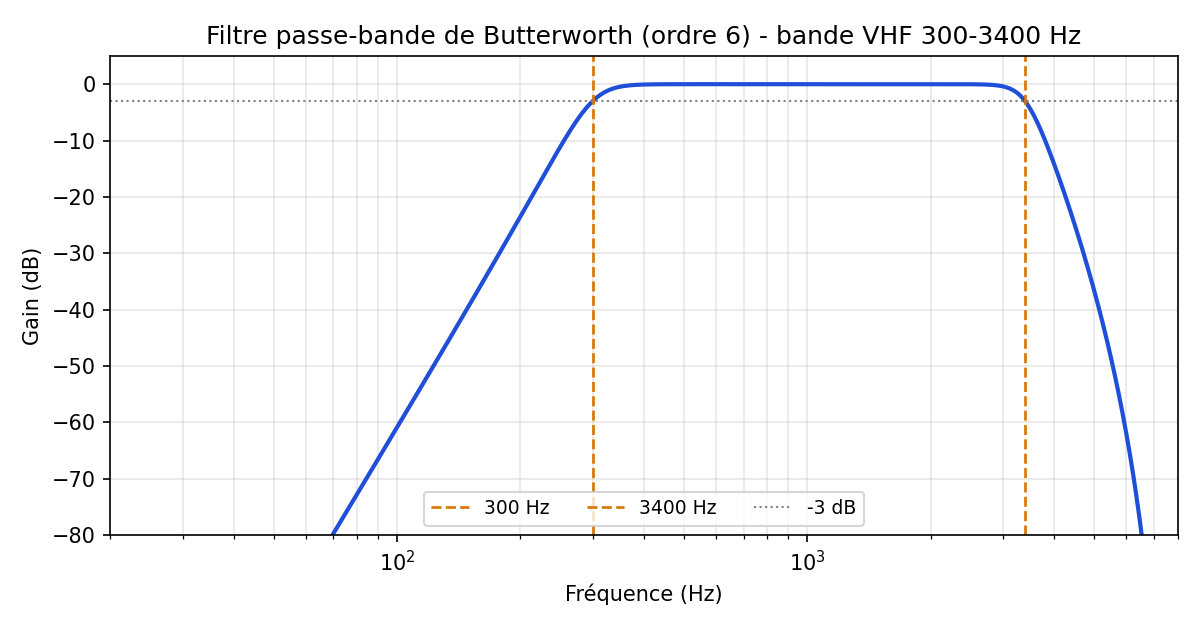
\includegraphics[width=0.70\textwidth]{figures/fig_butterworth_bode.png}
\caption{Reponse en frequence du filtre passe-bande de Butterworth (ordre~6) utilise
pour la degradation VHF. La bande utile est limitee a 300--3400~Hz, comme une radio
aeronautique.}
\label{fig:bode}
\end{figure}

\begin{figure}[h]
\centering
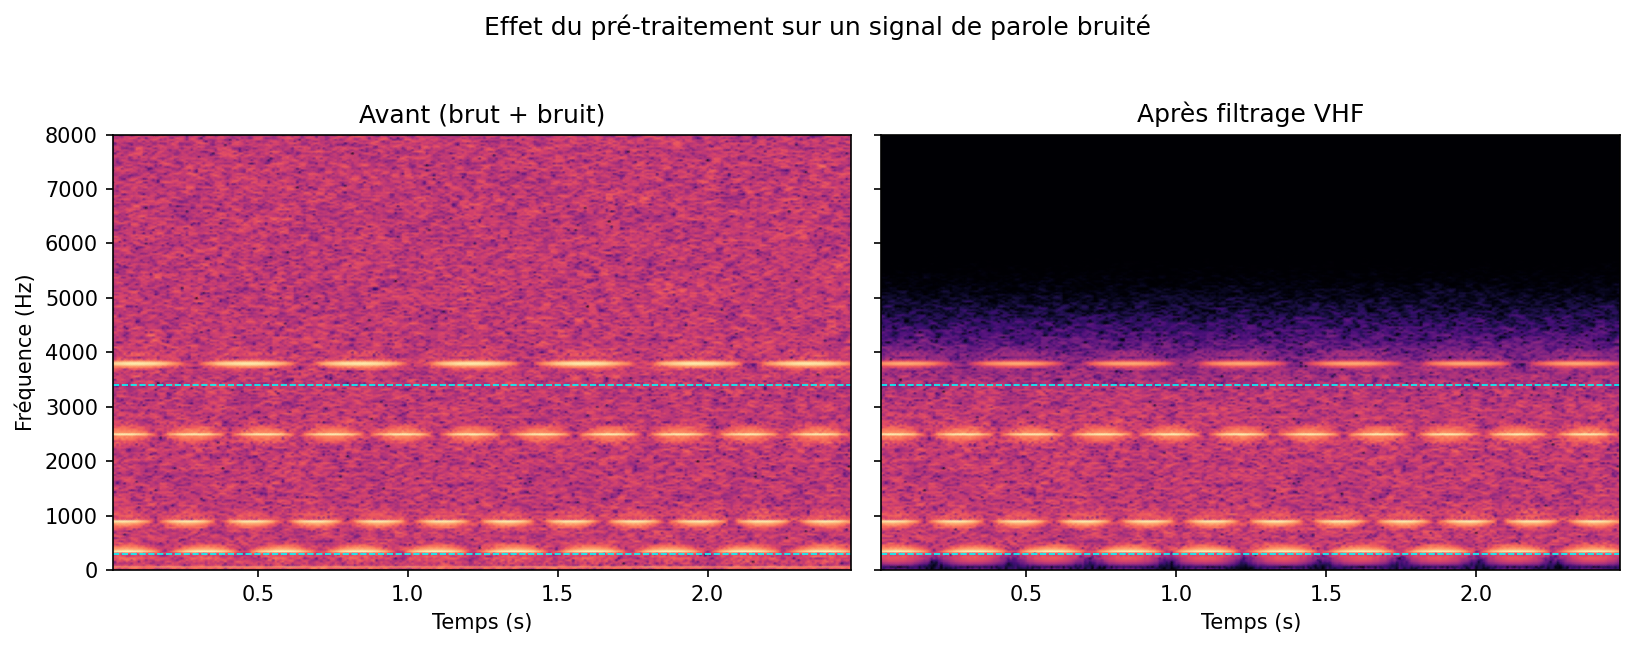
\includegraphics[width=0.84\textwidth]{figures/fig_spectrogramme_avant_apres.png}
\caption{Effet de la degradation VHF sur un signal de parole : spectre avant (gauche)
et apres filtrage passe-bande (droite). Le contenu hors bande 300--3400~Hz est
attenue, reproduisant la coloration d'un canal radio. La meme chaine est appliquee a
la voix synthetisee.}
\label{fig:spectro}
\end{figure}

\begin{warnbox}
L'integration de XTTS dans l'environnement logiciel du cluster a necessite plusieurs
ajustements. Le paquet \texttt{coqui-tts} a ete ajoute a l'environnement existant
(\emph{whisper-atc}) plutot que dans un environnement separe, afin de reutiliser la
meme version de PyTorch et de \texttt{transformers} : ce choix evite une seconde
installation de PyTorch, tient dans le quota disque de 20~Go et permet de servir les
trois modeles (Whisper, Mistral, XTTS) depuis un unique processus. Comme XTTS importe
un symbole (\texttt{isin\_mps\_friendly}) supprime dans \texttt{transformers} 5.x, ce
symbole est restaure par un correctif applique avant l'import de la bibliotheque, sans
retrograder \texttt{transformers} (qui doit rester en version~5.9 pour Whisper et
Mistral). Enfin, l'encodeur de locuteur de XTTS declenche un bug cuFFT de
\texttt{torchaudio} sur le GPU GH200 ; la synthese est donc executee sur CPU, ce qui
la rend fiable mais non temps reel.
\end{warnbox}

\subsection{La boucle vocale complete}

L'assemblage est valide par le module \texttt{voice\_exchange.py}, qui rejoue un
echange radio complet. Pour chaque instruction, le controleur parle (synthese~+~VHF),
l'audio est transcrit puis interprete, BlueSky execute l'ordre, et l'aeronef
collationne dans \emph{sa} voix clonee (synthese~+~VHF). Le collationnement est ensuite
re-transcrit pour verifier son intelligibilite, et les signaux sont assembles en
fichiers d'echange et en une bande son de session. La boucle complete
\emph{voix~$\rightarrow$~Whisper~$\rightarrow$~Mistral+RAG~$\rightarrow$~BlueSky~$\rightarrow$~readback vocal}
a ete rejouee et verifiee le 2026-06-11 (descente FL280~$\rightarrow$~FL180 executee
puis collationnee), comme l'illustre la figure~\ref{fig:romeo}.

\begin{figure}[h]
\centering
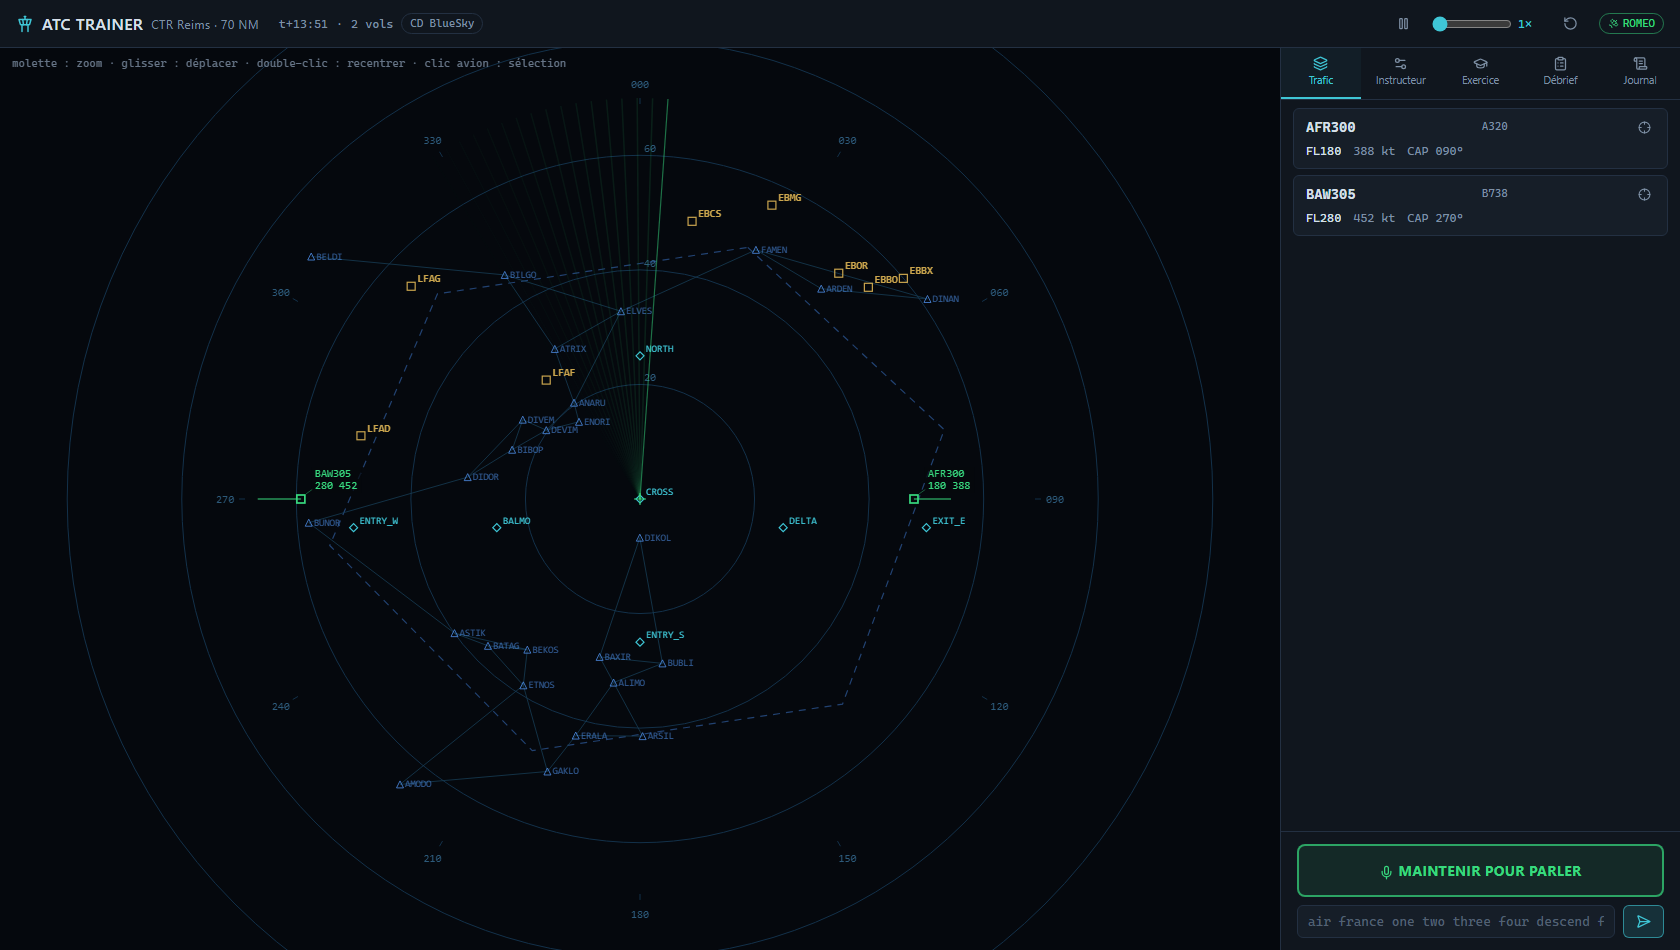
\includegraphics[width=0.92\textwidth]{figures/app_romeo.png}
\caption{Application en mode ROMEO : apres une clairance vocale, l'aeronef AFR300 est
etabli au FL180 et collationne dans sa voix clonee. La transcription de l'instruction
apparait sous le bouton \emph{push-to-talk}.}
\label{fig:romeo}
\end{figure}

\subsection{Resultats et mesures}

\begin{resbox}
\begin{itemize}
  \item \textbf{Latence de synthese} : 3,9~s par collationnement, facteur temps reel
  0,82 (XTTS sur CPU, n~=~3).
  \item \textbf{WER de re-transcription} de la voix synthetisee : 22 a 24~\% (mesure
  sur la boucle S6/S8).
  \item \textbf{Boucle vocale complete} rejouee et verifiee de bout en bout
  (2026-06-11).
  \item \textbf{Trois voix de reference} clonees, attribuees a des aeronefs distincts.
\end{itemize}
\end{resbox}

\noindent\textbf{Analyse.} La re-transcription de la voix synthetisee atteint un WER de
22 a 24~\%, contre 6,7~\% pour une voix humaine reelle (validation de la semaine~4).
Cet ecart est attendu : la boucle voix-clonee~$\rightarrow$~Whisper cumule les erreurs
de deux modeles successifs (la synthese et la reconnaissance), et la voix synthetique
presente des caracteristiques hors du domaine d'entrainement du module de
reconnaissance. Ce taux confirme neanmoins que le collationnement reste
\emph{intelligible} et exploitable pour un retour radio dans un contexte
d'entrainement. La synthese reste par ailleurs stochastique : sur un meme texte, une
generation propre et une generation plus degradee ont ete observees. Avec un facteur
temps reel de l'ordre de 0,82 sur CPU, la synthese n'autorise pas un flux continu en
temps reel, mais reste compatible avec le rythme d'une frequence reelle (un echange
toutes les dizaines de secondes).

%=============================================================================
\section{Semaine 7 : Integration -- la requete unifiee}
%=============================================================================

\begin{objbox}
Construire une requete unifiee prenant en entree la transcription, les regles du RAG
et une situation spatiale fixe, et produisant en sortie un JSON propre et exploitable
decrivant l'action a mener (\texttt{\{callsign, action, value, [wpt]\}}).
\end{objbox}

\subsection{Les trois entrees de la requete}

La requete unifiee agrege trois sources d'information complementaires :

\begin{itemize}
  \item \textbf{La transcription} : le texte de la clairance, issu du module de
  reconnaissance vocale (semaine~4) ou saisi directement.
  \item \textbf{Les regles du RAG} : les fiches de phraseologie les plus pertinentes
  pour cette clairance, recuperees par recherche vectorielle (semaine~5, $k = 4$).
  \item \textbf{La situation spatiale fixe} : une representation de l'espace aerien
  (le graphe de secteur), qui fournit au LLM la liste des points connus et la
  topologie, et qui sert ensuite a valider les ordres de routage.
\end{itemize}

\subsection{La situation spatiale fixe : le graphe de secteur}

La situation spatiale est decrite par un graphe statique du secteur, charge depuis
\texttt{secteur\_graphe.json}. Il comporte 7~points (de type \emph{entry}, \emph{fix}
ou \emph{exit}), 6~segments orientes avec leur distance, et une separation imposee de
5~NM (figure~\ref{fig:graphe}). La classe \texttt{SectorGraph} expose la liste des
fixes, le voisinage, le plus court chemin (Dijkstra sur les distances) et un resume
textuel compact de la topologie. C'est ce resume qui est injecte dans la requete pour
donner au LLM une conscience spatiale, sans alourdir le \emph{prompt}.

\begin{lstlisting}[caption={Resume textuel de la topologie injecte dans la requete (\texttt{topology\_text()}).}]
Sector (separation 5.0 NM).
Fixes: ENTRY_W(entry), BALMO(fix), CROSS(fix), DELTA(fix), EXIT_E(exit), ENTRY_S(entry), NORTH(exit).
Segments: ENTRY_W-BALMO 25.0NM; BALMO-CROSS 25.5NM; CROSS-DELTA 25.5NM; CROSS-ENTRY_S 25.0NM; CROSS-NORTH 25.0NM; DELTA-EXIT_E 25.0NM.
\end{lstlisting}

\begin{figure}[h]
\centering
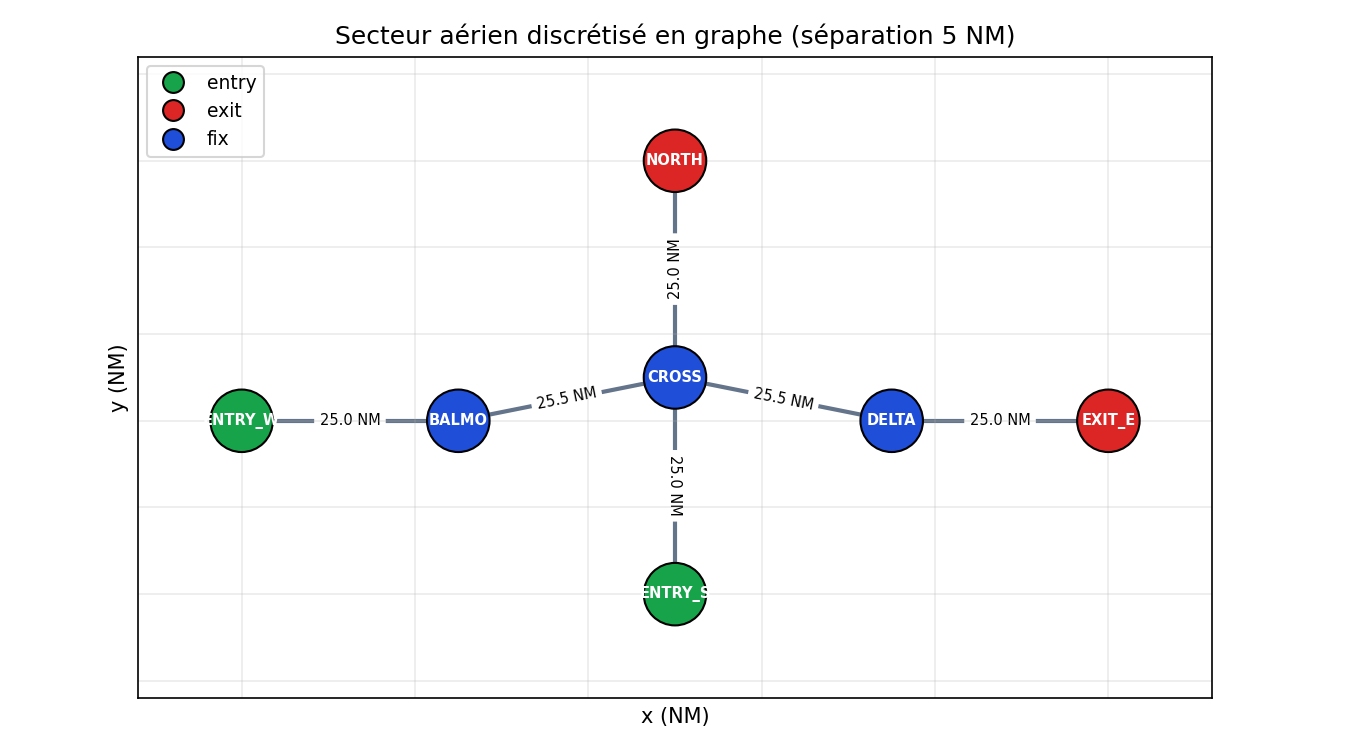
\includegraphics[width=0.64\textwidth]{figures/fig_secteur_graphe.png}
\caption{Situation spatiale fixe : le graphe du secteur (points d'entree, fixes,
sorties ; segments et distances). Il fournit le contexte spatial de la requete et
valide les ordres de routage. A ce stade, cette topologie est statique (sans etat de
trafic).}
\label{fig:graphe}
\end{figure}

\subsection{Construction de la requete unifiee}

La fonction \texttt{build\_messages} assemble les trois entrees en un unique message
adresse au LLM, precede d'un \emph{prompt} systeme strict qui impose une sortie au
format JSON et seulement cela. Les regles recuperees, la topologie du secteur, les
indices d'entites (indicatif, intentions) et la transcription sont concatenes dans un
ordre fixe.

\begin{lstlisting}[language=Python, caption={Assemblage de la requete unifiee (extrait de \texttt{atc\_llm.py}).}]
rules  = "\n".join(f"- {d['title']}: {d['text']}" for d, _ in retrieved)
sector = f"Sector graph: {graph.topology_text()}\n\n"
hint   = f"callsign={ner_callsign}; intentions_detectees={ner_intentions}"
user = (f"Applicable ICAO phraseology rules:\n{rules}\n\n"
        f"{sector}"
        f"NER hints: {hint}\n\n"
        f"Controller transcription: \"{transcription}\"\n\n"
        "Return ONLY the JSON array of orders.")
messages = [{"role": "system", "content": SYSTEM}, {"role": "user", "content": user}]
\end{lstlisting}

Sur un exemple, la requete assemblee et la sortie attendue prennent la forme suivante :

\begin{lstlisting}[caption={Requete unifiee assemblee (abregee) et JSON produit par le LLM.}]
Applicable ICAO phraseology rules:
- Instruction de cap (heading): ... action HDG, value = cap en degres ...

Sector graph: Sector (separation 5.0 NM). Fixes: ENTRY_W(entry), BALMO(fix), ...

NER hints: callsign=AFR1234; intentions_detectees=['turn']

Controller transcription: "air france one two three four turn right heading two seven zero"

Return ONLY the JSON array of orders.
-->  [{"callsign": "AFR1234", "action": "HDG", "value": 270}]
\end{lstlisting}

\subsection{Orchestration : de la transcription au JSON}

La fonction \texttt{interpret()} enchaine les etapes de la requete unifiee : extraction
des entites (NER) pour l'indicatif et les intentions, recuperation des $k = 4$ fiches
pertinentes, assemblage de la requete, generation par le LLM (Mistral~7B), puis analyse
tolerante du JSON et validation. La sortie est une liste d'ordres structures, chacun
associe a sa traduction executable ou a un motif de rejet.

\subsection{Garantir un JSON propre et exploitable}

L'integration ne se limite pas a produire du JSON : elle doit produire du JSON
\emph{exploitable sans risque}. Quatre verifications deterministes s'appliquent en aval
de la generation.

\begin{enumerate}[label=\textbf{\arabic*.}, leftmargin=2.0em]
  \item \textbf{Schema et bornes} : chaque ordre est traduit par
  \texttt{json\_to\_trafscript} ; toute valeur hors bornes (HDG 0--360, ALT 0--45000,
  SPD 0--350) ou action inconnue est rejetee.
  \item \textbf{Coherence spatiale} : un ordre de routage (\texttt{ADDWPT}) doit cibler
  un fix \emph{connu} du secteur, sinon il est rejete ou normalise vers le fix correct.
  \item \textbf{Coherence semantique} : si la clairance dit ``descend'' (sans
  ``climb'') mais que l'ordre vise un niveau \emph{au-dessus} du niveau actuel de
  l'aeronef, l'ordre est juge incoherent (transcription tronquee ou hallucination) et
  rejete plutot qu'execute ; le critere est symetrique pour ``climb''.
  \item \textbf{Realisme radio} : un ordre adresse a un indicatif absent du radar ne
  produit aucune reponse et n'est pas transmis au simulateur.
\end{enumerate}

\begin{warnbox}
A ce stade de l'integration, la situation spatiale fournie au LLM est volontairement
\emph{statique} : seule la topologie du secteur est injectee, pas encore l'etat de
trafic (positions et niveaux des aeronefs), qui fera l'objet de l'etape suivante. La
topologie est transmise sous forme d'un resume textuel compact plutot que du JSON
complet du graphe, afin de limiter la taille de la requete et de ne pas diluer
l'instruction. Le \emph{prompt} systeme reste strict pour que l'ajout du bloc spatial
ne pousse pas le modele a commenter sa reponse : seule la liste JSON est demandee, et
une analyse tolerante recupere le tableau meme si le modele ajoute du texte. La
verification de coherence semantique requiert l'altitude courante de l'aeronef ; elle
s'applique donc au moment de l'execution, lorsque cet etat est disponible.
\end{warnbox}

\subsection{Resultats et mesures}

\begin{resbox}
\begin{itemize}
  \item \textbf{Requete unifiee} operationnelle : transcription, regles RAG et
  situation spatiale fixe combinees en une seule passe vers le LLM.
  \item \textbf{JSON exploitable} produit sur 40 transcriptions reelles : 100~\%.
  \item \textbf{Validation de routage} : un \texttt{ADDWPT} vers un fix connu
  (\texttt{BALMO}) est accepte ; vers un point inconnu (\texttt{tango bravo}), il est
  rejete.
  \item \textbf{Garde-fou semantique} : une clairance tronquee de type ``descend flight
  level one'' qui ferait monter l'aeronef est detectee et rejetee.
\end{itemize}
\end{resbox}

\noindent\textbf{Analyse.} La requete unifiee atteint son objectif : sur les
transcriptions reelles evaluees, la sortie est systematiquement un JSON analysable, et
les quatre couches de validation eliminent les ordres dangereux, mal route ou
semantiquement incoherents avant toute execution. L'apport de l'integration ne tient
pas seulement a l'ajout du contexte spatial, mais aussi a la \emph{convergence} des
verifications en un point unique : un meme ordre est confronte aux bornes physiques, a
la topologie du secteur et a la coherence de l'instruction. La principale limite a ce
stade est que la conscience spatiale du LLM reste statique : il connait la geometrie du
secteur mais pas la position courante des aeronefs. C'est cette derniere information qui
permettra, ensuite, des decisions reellement situees (anticipation de conflit, routage
tenant compte du trafic).

%=============================================================================
\section{Bilan et transition}
%=============================================================================

Les semaines~6 et~7 marquent deux progressions complementaires. La semaine~6 complete
la boucle de dialogue par un module de restitution vocale : le clonage \emph{zero-shot}
XTTS-v2 genere a la volee une voix distincte par aeronef sans entrainement par
locuteur, et la degradation VHF reutilisee de la semaine~2 assure a la fois le realisme
radio et la coherence de domaine avec le module de reconnaissance. La semaine~7 etablit
le socle de l'integration : une requete unifiee combine la transcription, les regles du
RAG et une situation spatiale fixe, et produit un JSON propre et exploitable decrivant
l'action a mener, fiabilise par quatre verifications deterministes appliquees en aval du
LLM (bornes, coherence spatiale, coherence semantique, presence au radar).

\medskip
\noindent\textbf{Prochaines etapes.} L'etape directe consiste a remplacer la situation
spatiale \emph{fixe} par l'etat de trafic \emph{courant} (positions et niveaux des
aeronefs), afin de passer d'une conscience spatiale statique a une conscience situee.
Suivront la consolidation de la boucle temps reel de bout en bout et une evaluation
quantitative sur des scenarios complets.

\end{document}
